\documentclass{bioinfo}
\copyrightyear{2014}
\pubyear{2014}

\usepackage{listings}

\begin{document}
\firstpage{1}

\title[short Title]{Adding versatility to Galaxy with the Dockerized integration of IPython}
\author[Sample \textit{et~al}]{Eric Rasche\,$^{2}$, Torsten Houwaart\,$^{1}$, John Chilton\,$^{3}$, Bj\"orn A. Gr\"uning\,$^{1}$ and Rolf Backofen\,$^{1}$\,\footnote{to whom correspondence should be addressed}}
\address{$^{1}$Bioinformatics Group, Department of Computer Science, University of Freiburg\\
$^{2}$Center for Phage Technology, Texas A\&M University\\
$^{3}$Department of Biochemistry and Molecular Biology, Penn State University}


\history{Received on XXXXX; revised on XXXXX; accepted on XXXXX}

\editor{Associate Editor: XXXXXXX}

\maketitle

\begin{abstract}

\section{Summary:}
The Galaxy Tool Shed enables easy installation, dependency management, and updates of tools in the Galaxy ecosystem. 
However, if tools are not available in the Galaxy Tool Shed, a Galaxy administrator often cannot help a user directly. 
This forces the user to download their data and leave the Galaxy environment for further analysis. The integration of 
IPython in Galaxy allows for analysis of data within the Galaxy framework with the full versatility of Python and its 
scientific libraries. This bridges the gap between users with programming experience and Galaxy by adding the flexibility 
of quickly prototyping solutions' problems and doing data analysis, while staying within the context of the Galaxy 
framework and retaining the large toolset already available. IPython is executed in a Docker container which is 
invoked and terminated automatically. This design provides a secure framework for the user and the Galaxy system.


\section{Availability and implementation:}
The integration of IPython in Galaxy was accomplished via the Galaxy Interactive Environment Framework. 
Notebook level security is provided by IPython isolation within a Docker container. This Galaxy plugin 
is freely available under the MIT License and can be downloaded from https://github.com/bgruening/galaxy-ipython. 
The Docker image is hosted on Docker Hub under bgruening/docker-ipython-notebook and is used automatically by the plugin.

\section{Contact:} \href{gruening@informatik.uni-freiburg.de}{gruening@informatik.uni-freiburg.de}
\end{abstract}

\section{Introduction}


The Galaxy platform \citep{Blank2010,Giardine2005,Goecks2010} has made advanced bioinformatics software accessible
to life scientists for many years. Galaxy has a default set of analysis tools and can be extended with additional
tools by locally produced tools, or by using the community driven collections of tools available from the Galaxy Tool Shed
\citep{Blankenber2014}. This approach to extend Galaxy and adding new data analysis tools to a Galaxy instance is sufficient
in most cases, but a more flexible tool allowing for a more tailored analysis may be needed.
In this work the IPython Galaxy project is introduced by extending the Galaxy framework with an interface to an
IPython \citep{Perez2007} instance running inside a Docker container.
IPython provides a web service which allows for a graphical and interactive way to compute and visualize data, 
extensible through publicly available Python libraries. The IPython instance is run within a Docker container, 
which isolates the written code from the rest of the system and provides security for both the user and the Galaxy instance. Finally, by providing and encouraging a route for arbitrary data analysis to be accomplished within the Galaxy framework, 
IPython notebooks allow for saved and embedded logs of analysis, furthering the ultimate goal of research reproducibility.



\begin{methods}
\section{Methods}

IPython is integrated as an interactive environment (IE) in Galaxy. The program flow is sketched as a diagram in 
figure~\ref{fig:diagram}. An interactive environment plugin primarily consists of a python Mako template file and some
associated configuration data. The configuration of the plugin allows for additional security constraints which is useful
for production instances. The plugin can be forced to send data using SSL and to use password authentication.
Additionally, the name of a custom Docker image can be provided in the configuration. This image will be downloaded and 
installed from the Docker Hub. The default Docker image is specially crafted to use in conjunction with the IPython plugin
and will be described in more detail later. The configuration is also responsible for providing a history data set 
association (HDA) for the template file in order to get access to the data. \\
The template file of the plugin is written in Mako, a Python template engine which can be used in conjunction with HTML
% RFY: Mako needs a reference
and Javascript code to generate web pages. In the first part of this plugin's template file, a configuration is generated with a password
and an API-key for the Docker container. These pieces of information are stored so that Galaxy
% RFY: Define API first time used
% ESR: I don't think this is necessary for our target audience? But maybe?
and the IPython web service, which will be started in the Docker container, can communicate while isolated from the rest of the server. 
% ESR: Can we use "Dockerized" here? If so, we can get rid of "which will...Docker container".
%This has to be rewritten, but I don't know how it works exactly.. IE can request port from Galaxy? 
% Most importantly a unique port is attributed to each Docker container so that different users using this plugin on the same server do not interfere with each other. \\

% RFY: I note taht there is an indent here but not at the start of other paragraphs. I recommend indenting every new paragraph
% ESR: Yes boss, but that's LaTeX and a configuration option, and not so important.
Once container configuration and other preparatory work are complete, the Docker container is launched with bi-directional
access to a temporary directory containing the necessary initialization information. The default Docker container is
custom built and works hand-in-hand with the plugin. The container is built on top of a basic Debian Wheezy installation,
% RFY: (indicated that we should remove the dash between custom and built)
% ESR: Huh, custom built is being automatically hyphenated. May need to replace with \~ or another phrasing, unless one of you know which package is doing that.
and provides a basic IPython server, with its dependencies and some extra Python libraries such as NumPy, SciPy and Matplotlib.
% RFY: reference numpy/scipy/matplotlib, all software packages used
% RFY: since these are proper names, they should be capitalized and/or referenced
By providing images with a full suite of Python scientific analysis tools and libraries, users are able 
to immediatly perform their intricate analysis and calculations. Additional Python packages can be installed with Python
package managers, e.g.\ pip. The same is true for R packages or anything that can be installed in a non-priviledged user account. 
% RFY: Same as above. Pip and R need to be referenced
The IPython notebook is then embedded inside the usual Galaxy interface and can be used to interactively program in Python.
Having abstracted the chosen container into a site-specific configuration option, Galaxy instances with different use cases
and needs can provide Docker images to their users with appropriate tool suites.\\
During Docker container startup, a cron job is launched which allows for determining whether or not the IPython service
% RFY: Cite cron
is still being used by checking the network traffic. If the page with the IPython notebook is closed, after a minute the
% RFY: "after a minute", literally 60 seconds or after a defined period of time?
Docker process automatically terminates itself. Furthermore, two important custom functions are defined which enable the
user to load data from the history or store data to the Galaxy history respectively using the Galaxy API \citep{Sloggett2013}.
The \textbf{\texttt{get}} function expects one parameter with the identifier of the data set which corresponds to the number
of the data set in the history. The \textbf{\texttt{put}} function automatically builds a connection to the host
Galaxy instance with the correct history ID and uploads a specified file inside the Docker container to the user's
history from which the IPython service was started. The flexibility of this plugin is obvious: any data set can be
loaded into the notebook, data sets can be combined or modified, and the results can be written back to the history
all without the need for the user to download and upload data. \\
% Lack of segue between "itself. Furthermore"
Upon starting the IPython IE a check is performed on the data set from which the IPython IE was called; compatible IPython
notebooks will be reused, while other datasets utilize a notebook generated from a template. It should be stressed that
this functionality ensures the reproducibility of data analysis performed with this plugin, and is therefore an essential
feature.
% RFY: This sentence is not clear to me. Of course, that may just reflect my ignorance. But if it is important, it should be a bit clearer?


\section{Use Cases}
\subsection{Plotting Data}
Prior to the existence of the Galaxy IPython plugin, if a user wanted to transform and plot a specific column of a dataset and
get the result in a file of the Scalable Vector Graphics (SVG) format to do further image manipulation,
the user would have to download the data set which could take a long time depending on the file size and their internet
connection, complete their plotting of the dataset and record their commands to make it reproducible.
The task of plotting seems trivial at first because there are several useful tools in the toolshed for data visualization,
however these fail to provide a user and research friendly workflow. With the use of the IPython IE plugin the user
could copy their data set inside the Docker container with the \texttt{get()} command. They can then manipulate the
data remotely with a fully functional Python shell, generate their plots, and finally store datasets and their notebooks.
This workflow reduces the input time and effort required on the end user significantly, the process of generating the plot
and exporting it as an SVG file becomes a matter of a few lines of Python and a couple of mouse clicks.

\lstset{language=python,
morekeywords={put, get}
}
\begin{lstlisting}[frame=single]
from matplotlib import pyplot as p
filename = get(57)
p.plotfile(filename,delimiter='\t',cols=(0,12))
p.savefig("col12.svg")
put("col12.svg")
\end{lstlisting}
In the code example the data set which has the ID 57 in the Galaxy history is loaded into the IPython notebook inside the
plotfile method of an matplolib.pyplot object. Of this file the 13th column is plotted against the first column and the
resulting plot is stored as a SVG file. The put command copies the image into the Galaxy history, so it is now persistently
stored and can be downloaded or shared like any other Galaxy object.

%TODO: Expand this section a LOT.
\subsection{API Interaction}
The implementation of the Galaxy IPython IE plugin is not designed to restrict the user, instead the intention is to free
them to do their analysis with best practices. To this end, the IPython Notebook provides direct access to a pre-configured
BioBlend object, allowing the user to make API calls as necessary. Having access to the API can be invaluable for running
batch analyses, launching multiple workflows over numerous datasets, etc. In order to respect security, information necessary
to accomplish this is stored outside of notebooks and available inside notebooks as static variables; the user is able to use
\texttt{API\_KEY} without displaying their API key, invaluable if the user intends to publishs their notebook as
part of their research effort.

%
%visualization plugin how implemented used because ease of integration
%
%config files provides history dataset association And general variables calls mako
%
%mako file mainly prepares a docker container with a configuration file and a notebook access url (with a specific docker port)
%invokes the docker container with
%
%API
%hist.id
%paswd
%conf.yaml
%
%mako template
%invoke docker
%command
%/import/configfile in docker
%runs ipython -> HTML object
%docker monitors tcp connections as cron job -> docker cleans up and kills itself
%
%IPython
%%predefined functions: get(datasetNr.) copy dataset into docker ocntainer .. example?
%%knows history_id
%put (filename,type)
%
%
%docker image what's in it
%
%put/get
%
%API key


\begin{figure}[!tpb]
\centerline{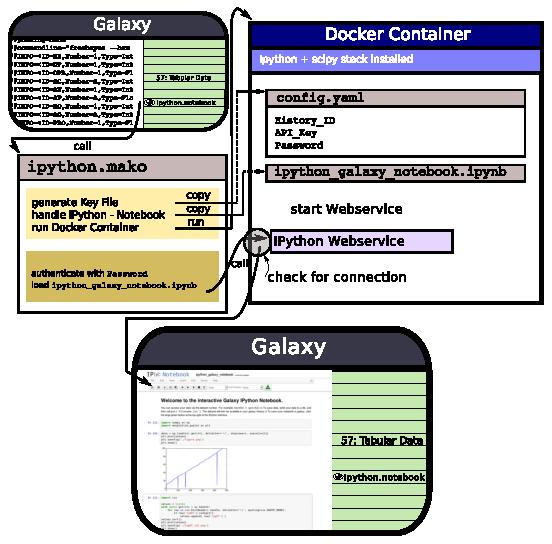
\includegraphics{diagram.pdf}}
\caption{Diagram of the program flow when the IPython IE is used. The IPython IE plugin is divided into two parts;
the first part generates initialization information and an IPython notebook, in the second part it launches a container
from a specific Docker image. In this Docker container, IPython and all its dependencies are installed as well as some Python
libraries. The configuration file and the IPython notebook are copied to the container and the IPython Webservice is started.
The second part of the IE template now generates a connection to the web service provided by the Docker container.
For self cleaning, the container also checks whether or not a connection to it exists, allowing the container to
terminate itself if it no longer in use.}
\label{fig:diagram}
\end{figure}


\end{methods}


%%%%%%%%%%%%%%%%%%%%%%%%%%%%%%%%%%%%%%%%%%%%%%%%%%%%%%%%%%%%%%%%%%%%%%%%%%%%%%%%%%%%%
%
%     please remove the " % " symbol from \centerline{\includegraphics{fig01.eps}}
%     as it may ignore the figures.
%
%%%%%%%%%%%%%%%%%%%%%%%%%%%%%%%%%%%%%%%%%%%%%%%%%%%%%%%%%%%%%%%%%%%%%%%%%%%%%%%%%%%%%%


\section{Conclusion}
The IPython-Docker container adds versatility to Galaxy by embedding a Python shell in a secure and easy to install manner.
This plugin represents a major shortcut for anybody with some programming experience who cannot wait for a specific tool to
be implemented in Galaxy or who needs more control to manipulate data. The possibilities with this plugin are immense and the
small example is just a glimpse of what could be done with a fully implemented scipy stack. The major security concern
of giving a user access to such a powerful tool as IPython, running on a Galaxy server, with the flexibility to install
packages as needed, has been resolved by running the IPython web service inside a Docker container. This sandboxes the user,
isolating them from the rest of the Galaxy server such that they can not break the system or read sensitive data from other
users. The user is additionally restricted by limits which administrators have placed on Docker containers,
hopefully preventing single users from launching denial of service attacks through over-use of memory/CPU cycles.
%TODO: Implement https://github.com/bgruening/galaxy-ipython/issues/24

The user can interact with the Galaxy instance via the two predefined functions \textit{put} and \textit{get} and these two
functions essentially define the exchange between the container and the Galaxy instance. With the possibility to store the
IPython notebook in the history, consistent and reproducible data analysis is possible and encouraged. 
By publishing or sharing a history containing IPython notebooks, notebooks can be easily shared with other users.
This way users with no programming experience can benefit from notebooks developed by users with programming experience.



\section*{Acknowledgement}
We would like to thank the Galaxy team and the Galaxy community for being so inspiring and helpful.


\paragraph{Funding\textcolon} The project was supported by the German Research Foundation (DFG-grant SFB 992/1).

\bibliographystyle{natbib}
%\bibliographystyle{achemnat}
%\bibliographystyle{plainnat}
%\bibliographystyle{abbrv}
%\bibliographystyle{bioinformatics}
%
%\bibliographystyle{plain}
%
%\bibliography{Document}


\begin{thebibliography}{}
\bibitem[Blankenberg {\it et~al}., 2010]{Blank2010}
Blankenberg, A. {\it et~al}., (2010) Galaxy: a web-based genome analysis tool for experimentalists. \textit{Curr. Protoc. Mol. Biol.},  {\bf Chapter 19}, Unit 19.10.1-21.

\bibitem[Giardine {\it et~al}., 2005]{Giardine2005}
Giardine, D. {\it et~al}., (2005) Galaxy: a platform for interactive large-scale genome analysis. \textit{Genome Res.},  {\bf 15}, 1451-1455.

\bibitem[Goecks {\it et~al}., 2010]{Goecks2010}
Goecks, J. {\it et~al}., (2005) Galaxy: a comprehensive approach for supporting accessible, reproducible, and transparent computational research in the life sciences. \textit{Genome Biol.},  {\bf 11}, R86.

\bibitem[P\'erez {\it et~al}., 2007]{Perez2007}
P\'erez, F. {\it et~al}., (2007) IPython: A System for Interactive Scientific Computing. \textit{Comput. Sci. Eng.}, {\bf 9}, 21-29.

\bibitem[Sloggett {\it et~al}., 2013]{Sloggett2013}
Sloggett, C. {\it et~al}., (2013) BioBlend: automating pipeline analyses within Galaxy and CloudMan. \textit{Bioinformatics}, {\bf 29}, 1685-1686.

\bibitem[Blankenberg {\it et~al}., 2014]{Blankenberg2014}
Blankenberg, A. {\it et~al}., (2014) Dissemination of scientific software with Galaxy ToolShed. \textit{Genome Biol.}, {\bf 15}, 403.



\end{thebibliography}
\end{document}
